

For this thesis, we showed Schasfoort several regions from the dataset during prominent drought periods and asked for her expert opinion on why these impacts might have occurred. This helped us explain and validate the identified drought impacts, while also creating a narrative around the dataset to better understand the underlying causes of the observed events.

For the selected time periods, we focused on the drought of 2022, for which Schasfoort contributed to an expert report for Deltares and was responsible for integrating different perspectives. We also selected the most recent drought event in our dataset, namely 2025. This period was selected because it represents the most recent conditions, meaning that current management practices and system characteristics are likely more comparable to future drought events. Therefore, this period may provide insights that are relevant for understanding future drought impacts.

\begin{figure}[htps!]
    \centering
    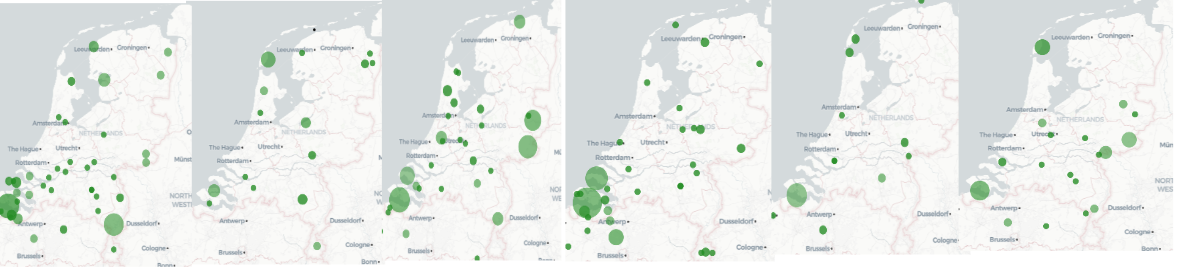
\includegraphics[width=1\linewidth]{figures/Agriculutre 2022 and 2025 may jun jul.png}
    \caption{Agricultural drought impacts reported in newspaper articles in Zeeland during the drought periods of 2022 and 2025 (May--July).}
    \label{fig:agriculture-zeeland}
\end{figure}

When observing the time series of Agricultural drought impacts(Figure~\ref{fig:agriculture-zeeland}), we consistently observe a high number of newspaper reports in Zeeland. These reports contain drought impacts such as: "Driekwart van de boeren in Zeeland heeft echter geen toegang tot zoet water" and "boeren in Zeeland moesten zoetwater aanvoeren met vrachtwagens". According to Femke Schasfoort, this pattern is logical because salinisation is a larger challenge in Zeeland compared to other regions of the Netherlands. The region is highly vulnerable due to its dependence on rainfall as a freshwater source. During drought conditions, freshwater availability becomes limited, and additional measures such as freshwater transport by trucks may be required. Therefore, the observed reporting pattern in our dataset aligns with the expected drought impact mechanisms.

\begin{figure}[htps!]
    \centering
    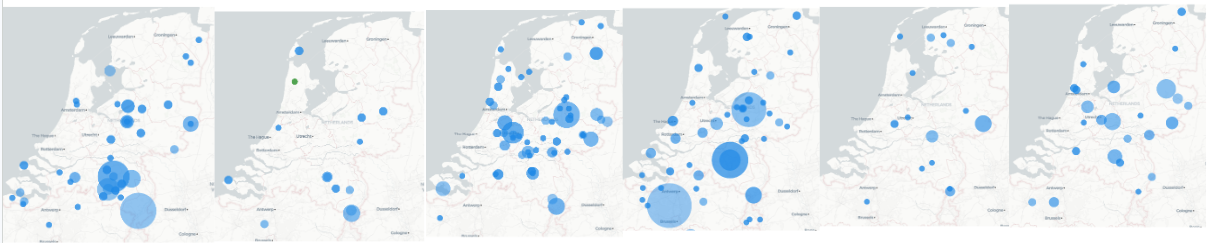
\includegraphics[width=1\linewidth]{figures/Hydrological 2022 and 2025 may jun jul.png}
    \caption{Hydrological drought impacts reported in newspaper articles in Overijssel and Brabant during the drought periods of 2022 and 2025 (May--July).}
    \label{fig:hydrological-overijssel-brabant}
\end{figure}

We also showed Femke a time series of hydrological impacts (Figure~\ref{fig:hydrological-overijssel-brabant}). In Overijssel and Brabant, we observe structurally more newspaper-reported drought impacts compared to other regions. These impacts include groundwater depletion, reservoir and surface water shortages, water use restrictions, and water supply and sanitation issues. Schasfoort explained that the higher impact levels in these regions are related to their physical characteristics. Figure~\ref{fig:soil-type} shows that these areas mainly consist of sandy soils and are relatively elevated compared to other parts of the Netherlands. During droughts or prolonged periods without rainfall, these regions are more difficult to supply with sufficient water. Maintaining freshwater availability requires additional measures, such as pumping water towards elevated areas. Therefore, it is expected that these regions appear as drought impact hotspots in the dataset.

These observations provide validation for the drought impact database. The identified impacts in different domains consistently align with expert knowledge and are supported by logical causal mechanisms.

Schasfoort also mentioned that drought impacts on water-dependent sectors, such as shipping, could provide valuable insights for Deltares. However, after further investigation, we concluded that existing models specifically designed for these applications would likely provide more added value. Schasfoort further highlighted that the ecological consequences of droughts remain a relatively unexplored area for Deltares and governmental agencies. Building upon this observation, we focus the further analysis of the dataset on extracting additional insights into drought impacts on ecological systems, rather than manually investigating individual drought events.